\chapter{Considerações finais}


Como exposto por este trabalho, a robótica educacional apoia o aprendizado do aluno de forma multidisciplinar, colaborando no desenvolvimento motor, intelectual e social. Para os universitários, a robótica é um apoio para o aprendizado de áreas relacionadas à inteligência artificial, como a otimização. O algoritmo guloso e a programação dinâmica são exemplos de algoritmos trabalhados pela inteligência artificial para a resolução de problemas de otimização. Nas bibliografias, a implementação dos algoritmos de otimização é geralmente feita em liguagens como C e C++. Pouca referência é encontrada para implementações na linguagem Prolog, sendo esse um dos obstáculos no desenvolvimento deste projeto. 

A robótica é trabalhada na Universidade de forma heterogênia, com diversos tipos de hardware e software. O estudo desses vários tipos de hardware serviu de insumo para a decisão de se trabalhar com o kit Lego Mindstorms NXT neste projeto. Na definição das ferramentas utilizadas por este projeto teve-se o cuidado de buscar ferramentas que apoiassem não só à implementação, mas também a gerência de todo o projeto. 

Como citado anteriormente, para o levantamento da solução da questão de pesquisa utilizou-se um modelo de pesquisa híbrida exploratória/experimental que apoiou a definição da proposta inicial de trabalho, o levantamento bibliográfico, e a prova de conceito. Para apoiar a construção da máquina de raciocínio será utilizado um modelo de pesquisa híbrido exploratória-descritiva.

A proposta de construção de uma máquina de raciocínio, implementada em Prolog segundo um algoritmo de programação dinâmica, que otimize a execução de missões pelo robô, provou-se viável através da prova de conceito exposta neste trabalho. A Figura \ref{status} mostra a porcentagem de conclusão das tarefas previstas no cronograma.



\FloatBarrier
\begin{figure}[!h]
\centering
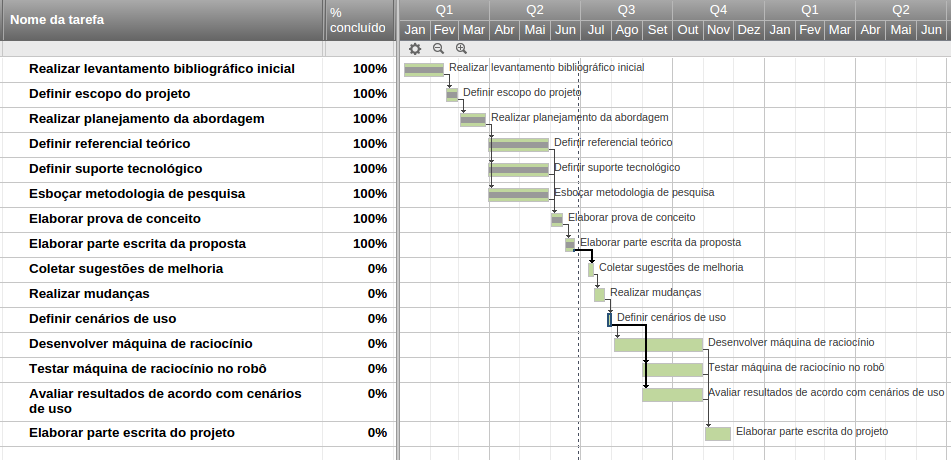
\includegraphics[keepaspectratio=true,scale=0.5]{figuras/status.png}
\caption{Status das atividades previstas pelo cronograma}
\label{status}
\end{figure}
 
Como na Faculdade do Gama o trabalho de conclusão de curso 02 tem um valor de créditos maior que o trabalho de conclusão de curso 01, assumiu-se que as tarefas previstas no cronograma para o TCC 01 tem um peso 1 e as previstas para o TCC 02 tem peso 1,5. Estes pesos são utilizados para calcular a porcentagem de conclusão do TCC como um todo, como mostra a Figura \ref{TCC}.

\FloatBarrier
\begin{figure}[!h]
\centering
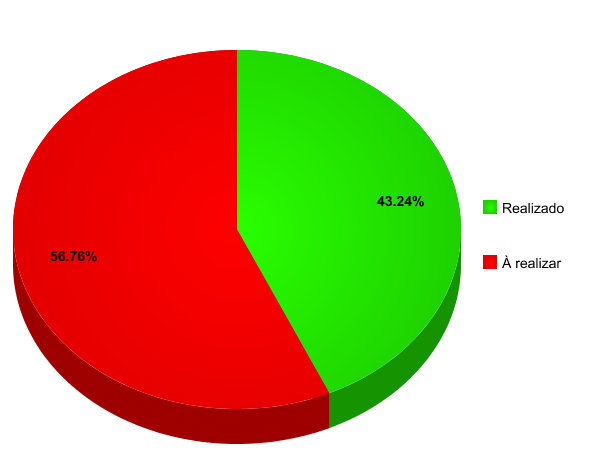
\includegraphics[keepaspectratio=true,scale=0.5]{figuras/TCC.png}
\caption{Status do projeto}
\label{TCC}
\end{figure}

A preocupação do TCC agora é lidar com a conexão via \textit{bluetooth} utilizando a ferramenta PLNXT. Assim que tal conexão estiver funcinando corretamente, será implementada a adaptação do problema da mochila para o contexto do trabalho. Em meios digitais, existem muitos códigos de exemplo da resolução do problema da mochila, utilizando programação dinâmica e implementados em Prolog que servirão como base para a implementação da máquina de raciocínio. 